\documentclass{note}
\usepackage[table,optidef]{mypackage}

\renewcommand{\thefootnote}{\fnsymbol{footnote}}

\title{机器学习笔记}
\author{陈鸿峥}
\date{{\builddatemonth\today} \protect\footnote{\text{Build \builddate\today}}}%加了build

\begin{document}

\maketitle
\renewcommand{\thefootnote}{\arabic{footnote}}
\setcounter{footnote}{0}

\setcounter{tocdepth}{2}%设置深度
\tableofcontents

\bigskip\bigskip
本笔记对应周志华的《机器学习》(西瓜书)。

% !TEX root = main.tex

\section{计算机系统概述}
\subsection{计算模型}
\begin{itemize}
	\item 图灵机(1936)
	\item 冯诺依曼体系结构(1945)\footnote{非冯诺依曼体系结构:并行计算、量子计算、生物计算} --- 存储程序原理(\textbf{运算器}为中心)\\
	计算机采用\textbf{二进制}表示机器指令和数据,按照程序指令\textbf{顺序}执行
\begin{center}
\begin{tikzcd}
& & \text{存储器}\arrow{d} & & \\
\quad\arrow{r} & \text{输入设备}\arrow{r} & \text{运算器}\arrow{r}\arrow{d}\arrow{u} & \text{输出设备}\arrow{r} & \quad\\
& & \text{控制器}\arrow{u}\arrow{lu}\arrow{ru}\arrow[bend left]{uu} & &
\end{tikzcd}
\end{center}
而现在由于计算不是瓶颈,存储访问成为了瓶颈,故现代微机以\textbf{存储器}为中心
\begin{center}
\begin{tikzcd}
& & \text{运算器}\arrow{d} & & \\
\quad\arrow{r} & \text{输入设备}\arrow{r} & \text{存储器}\arrow{r}\arrow{d}\arrow{u} & \text{输出设备}\arrow{r} & \quad\\
& & \text{控制器}\arrow{u}\arrow{lu}\arrow{ru}\arrow[bend left]{uu} & &
\end{tikzcd}
\end{center}
\end{itemize}
[运算器、控制器](CPU)、存储器为计算机的核心,合称主机;外围设备,简称外设,指除主机外的其他设备,包括IO设备、外存等

计算机中的信息仍用二进制表示的原因:由物理器件性能决定
\begin{itemize}
	\item 二进制只有两种状态,容易找到具有2个稳定状态并且状态转换容易控制的物理器件(数字电路)
	\item 二进制编码运算规则简单
	\item 二进制的0、1与二值逻辑一致,容易实现逻辑运算
\end{itemize}
% There are two reasons computers use the binary system:
% 1.Two clearly distinct states that provide a safety range for reliability.
% 2.Least amount of necessary circuitry, which results in the least amount of space, energy consumption, and cost.

\subsection{计算机的发展历程}
按发展历程可分为:电子管、晶体管、集成电路、(超)大规模集成电路四代计算机
\par重大历史事件如下
\begin{center}
\begin{tabular}{|c|c|c|c|}
\hline
% 年份 & 姓名 & 事件 & 备注 \\
1904 & 弗莱明(Fleming) & 二极管 & \\\hline
1907 & 德福雷斯特(De Forest) & 三极管 & \\\hline
1938 & 香农(Shannon) & 布尔代数与二值电子器件(继电器) & 奠定数字电路基石 \\\hline
1946 & & 第一台通用计算机ENIAC & 十进制 \\\hline
1947 & \begin{tabular}{c}布莱顿(Brattain)\\
巴丁(Bardeen)\end{tabular} & 点接触晶体管 & \\\hline
1949 & 肖克利(Shockley) & 结型晶体管(1949) & 1956诺贝尔奖\\\hline
1950 & & 二进制和存储程序EDVAC & 实现冯诺依曼设想(组合进步) \\\hline
1958 & Jack Kilby & 集成电路 & 2000诺贝尔奖 \\\hline
1965 & Moore & 摩尔定律 & \begin{tabular}{c}
在价格不变的情况下,每18个月芯片上\\
晶体管数目翻倍,性能也提升一倍
\end{tabular}\\\hline
1971 & Intel & 第一款微处理器4004 & 10$\mu$m\\\hline
\end{tabular}
\end{center}

\subsubsection{单处理器(1971-2002)}
性能提升主要手段
\begin{itemize}
	\item 提升工作主频:KHz增长至GHz(生产工艺进步,流水线级数增加)
	\item 指令级并行(ILP)
\end{itemize}
\begin{proposition}[安迪-比尔定律]
Andy gives, Bill takes away. 安迪是原Intel CEO,比尔是原微软CEO,硬件厂商靠软件开发商用光自己提供的硬件资源得以生存
\end{proposition}
但遇到频率墙和功耗墙
\[\text{功耗(power)}\propto 1/2\times\text{CMOS电容}\times\text{电压}^2\times\text{转换(01)频率}\]
\par
2004年,Intel放弃4GHz Pentium4芯片开发,因无法解决散热问题,通过加快主频提升处理器性能的路走到尽头

\subsubsection{多核处理器(2005-)}
采用多核处理器不过是将硬件的问题丢到软件\footnote{“向多核的转变并不是因为我们在软件或体系结构技术上取得了中大突破而带来的。相反,这种转变是当单处理器体系结构发展遇到了难以克服的巨大障碍时,我们被迫作出的一种选择。”---Kurt Keutzer (UCB), \emph{The Landscape of Parallel Computing Research: A View from Berkeley}}
\begin{theorem}[阿姆达尔(Amdahl)定律]
\label{thm:amdahl}
\[\text{改进后的执行时间}=\text{受改进影响部分的执行时间}/\text{改进提高的倍数}+\text{不受影响的执行时间}\]
\[S_A=\frac{1}{s+(1-s)/N},\]
\end{theorem}
对计算机系统的某个部分采用并行优化措施后所获得的计算机性能的提高是有上限的,上限由串行部分所占的比例决定
\begin{theorem}[古斯塔夫森(Gustafson)定律]
\[S_G=(s'+p'\times N)/(s'+p')=N+(1-N)\times s',\]
其中,$s'$和$p'$为程序串行部分与可并行化部分在并行系统上执行的时间占总时间的比例,$N$为处理器数量,简便起见设总时间$s'+p'=1$
\end{theorem}
打破Amdahl定律\textbf{问题规模不变}的假设,任何足够大的任务都可以被有效地并行化,只要问题规模可扩展,并行所带来的加速比就可以扩展


\subsection{计算机系统的层次结构}
\begin{center}
\begin{tikzcd}
\text{高级语言层}\arrow{d}{}\\
\text{汇编语言层}\arrow{d}{}\\
\text{操作系统层}\arrow{d}{}\\
\text{指令系统层}\arrow{d}{}\\
\text{微体系结构层}\arrow{d}{}\\
\text{数字逻辑层}
\end{tikzcd}
\end{center}
程序编译运行过程:
\begin{center}
\begin{tikzcd}
\text{高级语言}\quad\arrow{r}{\text{预编译、编译}} & \quad\text{汇编语言}\arrow{r}{\text{汇编}} & \text{目标文件(二进制)}\arrow{r}{\text{链接}} & \text{可执行文件(二进制)}\arrow{d}{\text{加载}}\\
& & \text{电路上的电信号}\quad & \quad\text{二进制机器指令流(硬盘$\to$存储器)}\arrow[swap]{l}{\text{CPU取指译码}}
\end{tikzcd}
\end{center}
计算机内部工作过程:逐条执行加载到内存中的二进制机器指令流的过程

指令执行分为两个阶段,周期性重复性进行:
\begin{itemize}
	\item 取指阶段:CPU从内存中读取指令,程序计数器(PC)保存要被要被取出的\textbf{下一条}指令的地址,除非遇跳转指令,否则都加一个增量\footnote{程序计数器(Program Counter)是一个实际存在的寄存器吗? - Belleve的回答 - 知乎 \url{https://www.zhihu.com/question/22609253/answer/21965180} PC每次增加\textbf{一条指令的长度/寻址粒度},在MIPS中一条指令长4字节,寻址粒度1字节,故每次PC加4;而x86体系指令长度不定,每次增加量会变化}
	\item 执行阶段:对取出的指令译码后执行
\end{itemize}
软件系统可分为系统软件和应用软件

\subsection{计算机结构的八个想法}
\begin{enumerate}
	\item 摩尔(Moore)定律:集成电路资源每$18-24$个月翻倍
	\item 抽象(abstraction):简化设计
	\item 加速常用操作(Make common case fast):见定理\ref{thm:amdahl}
	\item 并行(parallelism)
	\item 流水线(pipelining)
	\item 预测(prediction)
	\item 内存等级制(hierarchy)
	\item 冗余实现可靠性(redundancy):检测故障及解决
\end{enumerate}

\subsection{基本指标}
表示计算机通信带宽时
\begin{center}
\begin{tabular}{ccccccc}\hline
KB(yte) & MB & GB & TB & PB & EB & ZB\\\hline
$10^3$ & $10^6$ & $10^9$ & $10^{12}$ & $10^{15}$ & $10^{18}$ & $10^{21}$\\\hline
\end{tabular}
\end{center}
表示计算机存储二进制时
\begin{center}
\begin{tabular}{ccccccc}\hline
KiB(yte) & MiB & GiB & TiB\\\hline
$2^{10}$ & $2^{20}$ & $2^{30}$ & $2^{40}$\\\hline
\end{tabular}
\end{center}
\begin{itemize}
	\item 位(bit/b):计算机处理、存储、传输信息的最小单位
	\item 字节(Byte/B) $1\text{ Byte}=8\text{ bit}$:现代计算机主存按字节编制,字节是最小可寻址单位
	\item 字(Word):表示被处理信息的单位,用来度量数据类型的宽度\footnote{字长是指CPU中\textbf{数据通路的宽度},等于CPU内部总线的宽度或运算器的位数或通用寄存器的宽度;字和字长的宽度可以一样,也可以不同,通常是字节的整数倍}
\end{itemize}
\par 一台32位的电脑,一个字等于4个字节,字长为32位;若字长为16位,则一个字等于2字节.
\par 4字节相当于8位16进制编码

\subsection{性能评价}
\label{subsec:performance}
CPU主频:对同一型号计算机,主频越高,完成指令一个执行步骤时间越短
\[\text{计算机的性能(Performance)}=1/\text{执行时间(Execution time)}\]
按照单位(量纲)进行换算即可
\[\begin{aligned}
\text{CPU执行时间(s)}&=\text{执行程序所需CPU时钟周期(cyc)}\times\text{时钟周期s/cyc)}\\
&=\text{指令数目(ins)}\times\text{CPI(cyc/ins)}\times\text{时钟周期(s/cyc)}
\end{aligned}\]
程序性能对执行事件的影响:
\begin{center}
\begin{tabular}{|c|c|c|c|}\hline
 & 指令数 & CPI & 时钟周期\\\hline
算法、编程语言、编译器 & $\times$ & $\times$ & \\\hline
指令集 & $\times$ & $\times$ & $\times$ \\\hline
计算机组成 & & $\times$ & $\times$ \\\hline
实现技术 & & & $\times$\\\hline
\end{tabular}
\end{center}
体系结构=指令集体系结构(功能定义与设计)+计算机组成(考虑用什么材料)\\
举例来说:
\begin{itemize}
	\item 指令集(ISA)考虑:是否提供乘法指令
	\item 组成(Organization)考虑:如何实现乘法指令(专门乘法器还是加法器+移位器)
	\item 实现技术(Technology)考虑:如何布线、用什么材料和工艺
\end{itemize}

% 带有处理器的设备一般称为智能化设备
% 完整的计算机系统应包括配套的硬件设备和软件系统
% !TEX root = main.tex

\section{基础概念}
\subsection{训练集与测试集}
\begin{itemize}
	\item 留出法(hold-out):直接将数据集划分为两个互斥的集合,一个作为训练集,另一个作为测试集
	\begin{itemize}
		\item 注意数据分布的一致性,通过多次随机划分取平均保证
		\item 通常用$2/3\thicksim 4/5$的样本用于训练,其余用作测试
	\end{itemize}
	\item 交叉验证法(cross validation)/$k$折(fold)交叉验证:划分为$k$个互斥子集,其中$k-1$个用于训练,最后一个用于验证,训练$k$次,对这$k$次结果取平均
	\begin{itemize}
		\item 通常采用10次10折交叉验证,每次都换划分方式,确保随机性
	\end{itemize}
	\item 自助法(bootstrapping):从原始数据集中放回采样得到新数据集作为测试集
	\begin{itemize}
		\item 在数据集较小的、难以有效划分训练/测试集时比较有用
		\item 但改变了初始数据集分布,会引入估计偏差
	\end{itemize}
\end{itemize}

注意:通常将习得模型实际使用中遇到的数据称为测试集,而将训练的数据划分为训练集与验证集(validation)

\subsection{参数选择}
参数通常包括
\begin{itemize}
	\item 模型本身的参数(parameter):通过学习改变
	\item 超参数(superparameter):预先设定,调参实际上就是在选择算法
\end{itemize}

\subsection{性能度量}
\begin{itemize}
\item 回归:通常采用均方误差(MSE)
\item 分类:错误率、精度
\end{itemize}

对于二分类问题,有混淆矩阵(confusion matrix)
\begin{center}
\begin{tabular}{|c|c|c|}\hline
& 预测正 & 预测反\\\hline
真实正 & TP(真正例) & FN(假反例)\\\hline
真实反 & FP(假正例) & TN(真反例)\\\hline
\end{tabular}
\end{center}
\[\begin{aligned}
\text{查准率}P&=\frac{TP}{TP+FP}\\
\text{查全率}R&=\frac{TP}{TP+FN}
\end{aligned}\]

为了衡量机器学习算法的泛化性能,需要知道以下指标:
\begin{itemize}
	\item 方差(variance):度量同样大小的训练集的变动所导致的学习性能的变化,即刻画数据扰动所造成的影响
	\[\Var{\vx}=\mathbb{E}_D\lrs{\lrp{f(\vx;D)-\bar{f}(\vx)}^2}\]
	\item 偏差(bias):度量学习算法的期望预测和真实结果的偏离程度,即刻画学习算法本身的拟合能力
	\[b^2(\vx)=\lrp{\bar{f}(\vx)-y}^2\]
	\item 噪声(noise):表达在当前任务上任何学习算法所能达到的期望泛化误差的下界
	\[\eps^2=\mathbb{E}_D\lrs{\lrp{y_D-y}^2}\]
\end{itemize}

泛化误差可以分解为
\[E(f;D)=b^2(\vx)+\Var{\vx}+\eps^2\]
即泛化性能是由学习算法的能力、数据的充分性及学习任务本身的难度决定的
\begin{figure}[H]
\centering
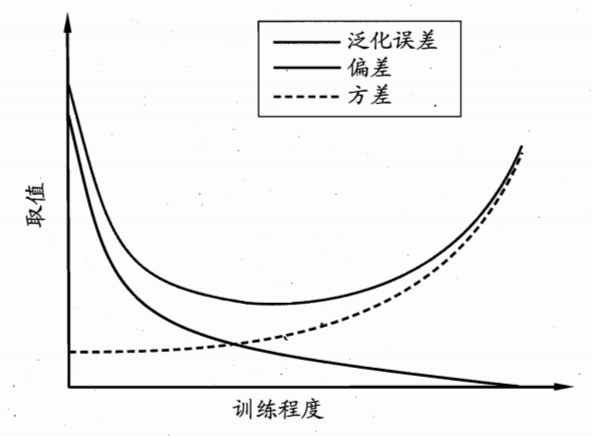
\includegraphics[width=0.4\linewidth]{fig/bias-var.png}
\end{figure}
% !TEX root = main.tex

\section{线性模型}
线性模型
\[f(\vx)=\vw^\T\vx+\vb\]
由于$\vw$直观表达了各属性在预测中的重要性,因此线性模型具有很好的可解释性(comprehensibility)。

\subsection{线性回归}
数据集$D=\{(\vx_i,y_i\}_{i=1}^m$,每个样本$\vx_i$都由$d$个属性描述,多元线性回归希望(multivariate linear regression)学到
\[f(\vx_i)=\vw^\T\vx_i+b,\;s.t.\,f(\vx_i)\simeq y_i\]

将$\vw$和$b$写在一起变成$\vw\gets\bmat{\vw & b}$,并设
\[X=\bmat{x_{11} & x_{12} & \cdots & x_{1d} & 1\\x_{21} & x_{22} & \cdots & x_{2d} & 1\\
\vdots & \vdots & \ddots & \vdots & \vdots\\x_{m1} & x_{m2} & \cdots & x_{md} & 1}=\bmat{\vx_1^\T & 1\\\vx_2^\T & 1\\\vdots & \vdots\\\vx^\T_m & 1}\]
为已知,$\vw$为需要训练的权重。
再将标记写成向量形式$\vy=\bmat{y_1 & y_2 &\cdots & y_m}$,进而得到最小二乘优化
\[\vw^\star=\argmin_\vw\norm{\vy-X\vw}_2^2\]

对$\vw$求导有
\[\nabla_\vw E_\vw=2X^\T(X\vw-\vy)\]
当$X^\T X$满秩或正定时,令上式为0有
\[\vw^\star=(X^\T X)^{-1} X^\T\vy\]
但现实中大多数时候$X^\T X$都非可逆阵,故常用正则化方法。

\subsection{线性分类}
单位阶跃(unit-step)函数
\[y=\begin{cases}
0 & z<0\\
0.5 & z=0\\
1 & z>1
\end{cases}\]
不连续,故用对数几率(logistic)函数替代
\[y=\frac{1}{1+\ee^{-z}}\]
这是一种Sigmoid函数,将线性表达式代入有
\[y=\frac{1}{1+\ee^{-(\vw^T\vx+b)}}\]
进而有
\[\vw^\T\vx+b=\ln\frac{y}{1-y}\]
将$y$视为样本$\vx$为正例的可能性,则$1-y$为反例可能性,两者比值$y/(1-y)$称为几率(odds),反映了$\vx$作为正例的相对可能性。
对数几率又称logit,故这种方法又称为逻辑斯蒂(logistic)回归,但其实是分类学习方法。

将$y$视为后验概率估计,有
\[\ln\frac{\prc{y=1}{\vx}}{\prc{y=0}{\vx}}=\vw^\T\vx+b\]
显然有
\[\begin{aligned}
\prc{y=1}{\vx}&=\frac{\ee^{\vw^\T+b}}{1+\ee^{\vw^\T\vx+b}}\\
\prc{y=0}{\vx}&=\frac{1}{1+\ee^{\vw^\T\vx+b}}
\end{aligned}\]

给定数据集$\{(\vx_i,y_i)\}_{i=1}^m$,由极大似然法估计$\vw$和$b$有
\[\ell(\vw,b)=\sum_{i=1}^m\ln\prc{y_i}{\vx_i;\,\vw,b}\]

\subsection{线性判别分析}
线性判别分析(Linear Discriminant Analysis, LDA)[Fisher, 1936]同样用于二分类,希望将样例投影到一条直线上,使得同类样例投影点尽可能近,异类样例投影点尽可能远。
\begin{figure}[H]
\centering
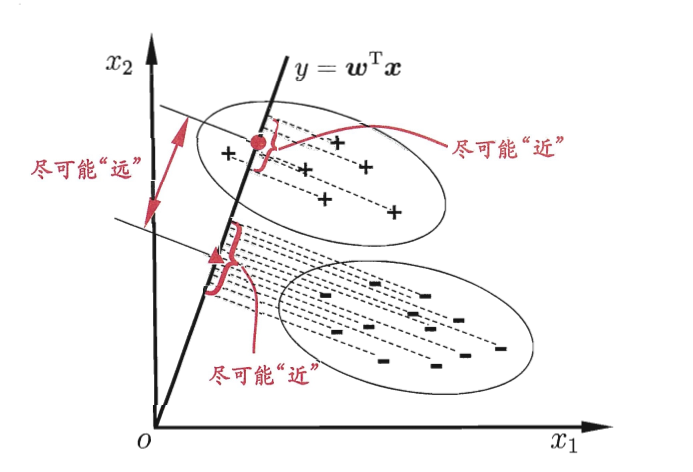
\includegraphics[width=0.5\linewidth]{fig/LDA.png}
\end{figure}

最优化广义瑞利商
\[J=\frac{\vw^\T S_b\vw}{\vw^\T S_w\vw}\]
其中$S_w$为类内散度矩阵,$S_b$为类间散度矩阵。

LDA也是经典的监督降维技术。

\subsection{类别不平衡问题}
\begin{itemize}
	\item 欠采样(undersampling):减少样例
	\item 过采样(oversampling):增加样例
	\item 阈值移动(threshold-moving)/再缩放(rescaling)
	\[\frac{y'}{1-y'}=\frac{y}{1-y}\times\frac{m^-}{m^+}\]
\end{itemize}
% !TEX root = main.tex

\section{参考资料}
\begin{enumerate}
	\item 周志华,《机器学习》,2016
	\item Jure Leskovec, Stanford CS246: Mining Massive Data Sets, \url{http://web.stanford.edu/class/cs246/}
\end{enumerate}

\end{document}